\hypertarget{privacy-datenschutz}{%
\section{Privacy \& Datenschutz}\label{privacy-datenschutz}}

\hypertarget{weshalb-privacy-und-datenschutz}{%
\subsection{Weshalb Privacy und
Datenschutz}\label{weshalb-privacy-und-datenschutz}}

Privatsphäre ist ein Menschenrecht. Alle modernen Demokratien schützen
diese! Im Grundsatz..

Um einen liberalen Lebensstil zu wahren, muss jeder Bürger selbst
entscheiden können \textbf{welche} Informationen er zur Verfügung stellt
und \textbf{wie} diese benutzt werden dürfen.

\hypertarget{sphuxe4rentheorie}{%
\subsection{Sphärentheorie}\label{sphuxe4rentheorie}}

\begin{figure}
\centering
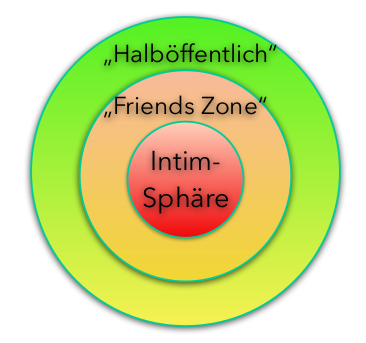
\includegraphics{figures/sphaerentheorie.png}
\caption{Sphärentheorie}
\end{figure}

Jeder entscheidet selbst, welche Daten/Information in welcher Sphäre
ist, weil jeder steht dazu was er macht.

\textbf{Persönlichkeitsverletzung}: Wenn Daten/Informationen von einer
Drittperson weitergegeben werden und somit ein Sphärenübertritt
stattfindet, spricht man von einer Persönlichkeitsverletzung.

\hypertarget{schutz-der-persuxf6nlichkeit}{%
\subsection{Schutz der
Persönlichkeit}\label{schutz-der-persuxf6nlichkeit}}

\begin{verbatim}
Wer in seiner Persönlichkeit widerrechtlich verletzt wird, kann zu seinem Schutz gegen jeden, der in der Verletzung mitwirkt, das Gericht  anrufen.
\end{verbatim}

\textbf{Sehr wichtig:}

\begin{verbatim}
Eine Verletzung ist widerrechtlich, wenn sie nicht durch Einwilligung des Verletzten, durch ein überwiegend privates oder öffentliches Interessen oder durch Gesetz gerechtfertigt ist.
\end{verbatim}

Dieses Gesetz stammt nicht vom Datenschutzgesetz, sondern vom
Zivilgesetzbuch.

Öffentliches Intresse besagt nicht, was die Öffentlichkeit
\textbf{interessiert} sondern was für die Öffentlichkeit
\textbf{relevant} ist.

\hypertarget{datenschutz}{%
\subsection{Datenschutz}\label{datenschutz}}

Als Datenschutz versteht man der Schutz der \textbf{Integrität} einer
Person vor Verletzungen Dritte.

Datenschutz ist\ldots{}

\begin{itemize}
\tightlist
\item
  Schutz der \textbf{informationellen Sebstbestimmung}
\item
  Schutz der Persönlichkeit bei der Datenverarbeitung
\item
  Schutz der Privatsphäre
\item
  Schutz vor missbräuchlicher Datenverbreitung
\end{itemize}

\hypertarget{gesetzliche-grundlagen}{%
\subsection{Gesetzliche Grundlagen}\label{gesetzliche-grundlagen}}

\begin{itemize}
\tightlist
\item
  Schweizerische Bundesverfassung
\item
  Bundesgesetz über den Datenschutz (DSG) und Verordnung dazu (VDSG)
\item
  Zahlreiche datenschutzrechtliche Bestimmungen in anderen Gesetzen
\item
  Kantonales und Gemeinderecht: zahlreiche Gesetze und Verordnungen
\item
  International: Europäische Datenschutzrichtlinie bzw. -Grundverordnung
  (DSGVO/GDPR)
\end{itemize}

\hypertarget{geltungsbereich-des-datenschutzgesetzes}{%
\subsection{Geltungsbereich des
Datenschutzgesetzes}\label{geltungsbereich-des-datenschutzgesetzes}}

Dieses Gesetz gilt für das Bearbeiten von Daten \textbf{natürlicher und
juristischer Personen} durch a. private Personen und b. Bundesorgane.

Es ist nicht anwendbar auf: - Personendaten, die eine \textbf{natürliche
Person ausschliesslich zum persönlichen Gebrauch bearbeitet und nicht an
Aussenstehende bekannt gibt} - Beratungen in den Eidgenössischen Räten
und in den parlamentarischen Kommissionen - \textbf{hängige
Zivilprozesse, Strafverfahren}, Verfahren der internationalen
Rechtshilfe sowie staats- und verwaltungsrechtliche Verfahren mit
Ausnahme erstinstanzlicher Verwaltungsverfahren - öffentliche Register
des Privatrechtsverkehrs - Personendaten, die das Internationale Komitee
vom Roten Kreuz bearbeitet.

\hypertarget{begriffe-definitionen}{%
\subsubsection{BEGRIFFE \& DEFINITIONEN}\label{begriffe-definitionen}}

\textbf{Personendaten} (Daten): alle Angaben, die sich auf eine
bestimmte oder bestimmbare Person beziehen.\\
\textbf{betroffene Personen}: natürliche oder juristische Personen, über
die Daten bearbeitet werden\\
\textbf{besonders schützenswerte Personendaten Daten} über\_\\
1. die religiösen, weltanschaulichen, politischen oder
gewerkschaftlichen Ansichten oder Tätigkeiten 42. die Gesundheit, die
Intimsphäre oder die Rassenzugehörigkeit, 42. Massnahmen der sozialen
Hilfe, 42. Massnahmen der sozialen Hilfe,

\textbf{Persönlichkeitsprofil}: Eine Zusammenstellung von Daten, die
eine Beurteilung wesentlicher Aspekte der\\
Persönlichkeit einer natürlichen Person erlaubt

\textbf{Bearbeiten}: jeder Umgang mit Personendaten, unabhängig von den
angewandten Mitteln und Verfahren, insbesondere das Beschaffen,
Aufbewahren, Verwenden, Umarbeiten, Bekanntgeben, Archivieren oder
Vernichten von Daten.

\textbf{Bekanntgeben}: das Zugänglichmachen von Personendaten wie das
Einsichtgewähren, Weitergeben oder Veröffentlichen.

\textbf{Datensammlung}: jeder Bestand von Personendaten, der so
aufgebaut ist, dass die Daten nach betroffenen Personen erschliessbar
sind.

\textbf{Bundesorgane}: Behörden und Dienststellen des Bundes sowie
Personen, soweit sie mit öffentlichen Aufgaben des Bundes betraut sind.

\textbf{Inhaber der Datensammlung}: private Personen oder Bundesorgane,
die über den Zweck und den Inhalt der Datensammlung entscheiden.

\hypertarget{datenschutzgrundsuxe4tze}{%
\subsubsection{DATENSCHUTZGRUNDSÄTZE}\label{datenschutzgrundsuxe4tze}}

\begin{enumerate}
\def\labelenumi{\arabic{enumi}.}
\tightlist
\item
  Personendaten dürfen nur \textbf{rechtmässig} bearbeitet werden.
\item
  Ihre Bearbeitung hat nach Treu und Glauben zu jerfolgen und muss
  \textbf{verhältnismässig} sein.
\item
  Personendaten dürfen \textbf{nur zu dem Zweck bearbeitet werden, der
  bei der Beschaffung angegeben wurde, aus den Umständen ersichtlich
  oder gesetzlich vorgesehen ist.}
\item
  Die Beschaffung von Personendaten und insbesondere der Zweck ihrer
  Bearbeitung müssen für die betroffene Person \textbf{erkennbar} sein.
\item
  Ist für die Bearbeitung von Personendaten die Einwilligung der
  betroffenen Person erforderlich, so ist diese Einwilligung erst
  gültig, wenn sie \textbf{nach angemessener Information freiwillig
  erfolgt}. Bei der Bearbeitung von besonders schützenswerten
  Personendaten oder Persönlichkeitsprofilen muss die Einwilligung zudem
  \textbf{ausdrücklich} erfolgen.
\end{enumerate}

\hypertarget{richtigkeit-der-daten}{%
\subsubsection{RICHTIGKEIT DER DATEN}\label{richtigkeit-der-daten}}

\begin{enumerate}
\def\labelenumi{\arabic{enumi}.}
\tightlist
\item
  Wer Personendaten bearbeitet, hat sich \textbf{über deren Richtigkeit
  zu vergewissern}. Er hat alle angemessenen Massnahmen zu treffen,
  damit die Daten \textbf{berichtigt oder vernichtet} werden, die im
  Hinblick auf den Zweck ihrer Beschaffung oder Bearbeitung unrichtig
  oder unvollständig sind.
\item
  \textbf{Jede betroffene Person kann verlangen, dass unrichtige Daten
  berichtigt werden}.
\end{enumerate}

\hypertarget{datensicherheit}{%
\subsubsection{DATENSICHERHEIT}\label{datensicherheit}}

\begin{enumerate}
\def\labelenumi{\arabic{enumi}.}
\tightlist
\item
  Personendaten müssen durch \textbf{angemessene technische und
  organisatorische} Massnahmen gegen \textbf{unbefugtes Bearbeiten}
  geschützt werden.
\item
  Der Bundesrat erlässt nähere Bestimmungen über die
  Mindestanforderungen an die Datensicherheit.
\end{enumerate}

\hypertarget{grenzuxfcberschreitende-bekanntgabe}{%
\subsubsection{GRENZÜBERSCHREITENDE
BEKANNTGABE}\label{grenzuxfcberschreitende-bekanntgabe}}

\begin{enumerate}
\def\labelenumi{\arabic{enumi}.}
\item
  Personendaten dürfen \textbf{nicht} ins \textbf{Ausland bekannt}
  gegeben werden, wenn dadurch die Persönlichkeit der betroffenen
  Personen \textbf{schwerwiegend gefährdet würde}, namentlich weil eine
  \textbf{Gesetzgebung} fehlt, die einen \textbf{angemessenen Schutz}
  gewährleistet.
\item
  \ldots{} zahlreiche Voraussetzungen bei fehlen einer schützenden
  Gesetzgebung (z.B. nach Wegfall „Safe Harbor``)
\end{enumerate}

\hypertarget{auskunftsrecht}{%
\subsubsection{AUSKUNFTSRECHT}\label{auskunftsrecht}}

\begin{enumerate}
\def\labelenumi{\arabic{enumi}.}
\item
  Jede Person kann vom Inhaber einer Datensammlung \textbf{Auskunft}
  darüber verlangen, \textbf{ob Daten über sie bearbeitet} werden.
\item
  Der Inhaber der Datensammlung \textbf{muss} der betroffenen Person
  \textbf{mitteilen}:

  \begin{itemize}
  \tightlist
  \item
    \textbf{alle} über sie in der Datensammlung \textbf{vorhandenen
    Daten} einschliesslich der verfügbaren Angaben über die
    \textbf{Herkunft} der Daten;
  \item
    den \textbf{Zweck} und gegebenenfalls die \textbf{Rechtsgrundlagen}
    des Bearbeitens sowie die Kategorien der bearbeiteten Personendaten,
    der an der Sammlung Beteiligten und der \textbf{Datenempfänger}.
  \end{itemize}
\item
  Daten über die Gesundheit kann der Inhaber der Datensammlung der
  betroffenen Person durch einen von ihr bezeichneten Arzt mitteilen
  lassen.
\item
  Lässt der Inhaber der Datensammlung Personendaten durch einen
  \textbf{Dritten bearbeiten}, so bleibt er \textbf{auskunftspflichtig}.
  Der Dritte ist auskunftspflichtig, wenn er den Inhaber nicht bekannt
  gibt oder dieser keinen Wohnsitz in der Schweiz hat.
\item
  Die Auskunft ist in der Regel \textbf{schriftlich}, in Form eines
  Ausdrucks oder einer Fotokopie sowie \textbf{kostenlos} zu erteilen.
  Der Bundesrat regelt die Ausnahmen.
\item
  \textbf{Niemand kann im Voraus auf das Auskunftsrecht verzichten.}
\end{enumerate}

\hypertarget{informationspflicht-beim-beschaffen-von-besonders-schuxfctzenswerten-personendaten-und-persuxf6nlichkeitsprofilen}{%
\subsubsection{INFORMATIONSPFLICHT BEIM BESCHAFFEN VON BESONDERS
SCHÜTZENSWERTEN PERSONENDATEN UND
PERSÖNLICHKEITSPROFILEN}\label{informationspflicht-beim-beschaffen-von-besonders-schuxfctzenswerten-personendaten-und-persuxf6nlichkeitsprofilen}}

\begin{enumerate}
\def\labelenumi{\arabic{enumi}.}
\tightlist
\item
  Der Inhaber der Datensammlung \textbf{ist verpflichtet}, die
  betroffene Person über die Beschaffung von besonders schützenswerten
  Personendaten oder Persönlichkeitsprofilen \textbf{zu informieren};
  diese Informationspflicht gilt auch dann, wenn die Daten bei Dritten
  beschafft werden.
\item
  Der betroffenen Person sind mindestens mitzuteilen:

  \begin{itemize}
  \tightlist
  \item
    der \textbf{Inhaber der Datensammlung};
  \item
    der \textbf{Zweck} des Bearbeitens;
  \item
    die \textbf{Kategorien der Datenempfänger}, wenn eine
    Datenbekanntgabe vorgesehen ist.
  \end{itemize}
\item
  Werden die Daten nicht bei der betroffenen Person beschafft, so hat
  deren Information \textbf{spätestens bei der Speicherung} der Daten
  oder, wenn die Daten nicht gespeichert werden, mit ihrer
  \textbf{ersten Bekanntgabe} an Dritte zu erfolgen.
\end{enumerate}

\ldots{}

\hypertarget{verletzung-der-auskunfts--melde--und-mitwirkungspflichten}{%
\subsubsection{VERLETZUNG DER AUSKUNFTS-, MELDE- UND
MITWIRKUNGSPFLICHTEN}\label{verletzung-der-auskunfts--melde--und-mitwirkungspflichten}}

\begin{enumerate}
\def\labelenumi{\arabic{enumi}.}
\tightlist
\item
  Mit \textbf{Busse} werden \textbf{private Personen} auf Antrag
  bestraft:

  \begin{itemize}
  \tightlist
  \item
    die ihre Pflichten nach den Artikeln 8--10 und 14 verletzen, indem
    sie vorsätzlich eine falsche oder eine unvollständige Auskunft
    erteilen.
  \item
    die es \textbf{vorsätzlich} unterlassen:

    \begin{itemize}
    \tightlist
    \item
      die betroffene Person nach Artikel 14 Absatz 1 zu informieren,
      oder
    \item
      ihr die Angaben nach Artikel 14 Absatz 2 zu liefern.
    \end{itemize}
  \end{itemize}
\item
  Mit Busse werden \textbf{private Personen} bestraft, die vorsätzlich:

  \begin{itemize}
  \tightlist
  \item
    die \textbf{Information} nach Artikel 6 Absatz 3 oder die
    \textbf{Meldung} nach Artikel 11a \textbf{unterlassen} oder dabei
    \textbf{vorsätzlich falsche Angaben machen};
  \item
    dem Beauftragten bei der Abklärung eines Sachverhaltes (Art. 29)
    \textbf{falsche Auskünfte} erteilen oder die \textbf{Mitwirkung}
    verweigern.
  \end{itemize}
\end{enumerate}

\hypertarget{beispiele}{%
\subsection{Beispiele}\label{beispiele}}

\hypertarget{ist-das-zuluxe4ssig}{%
\subsubsection{IST DAS ZULÄSSIG?}\label{ist-das-zuluxe4ssig}}

\textbf{Anonyme Mitarbeiterbefragung mit Altersangabe. 2 Personen im
Team sind 55plus.}\\
Nein. Die anonymen Daten dürfen nicht auf Personen zurückverfolgt werden
können.

\textbf{Die Personendaten werden verarbeitet: a) Deutschland, b) in den
USA und c) in der Türkei}

\begin{enumerate}
\def\labelenumi{\alph{enumi})}
\item
  Deutschland hat ein vergleichbaren Datenschutzgesetz, also is OK. Die
  europäische Datenschutzrichtlinien sind sogar noch härter.
\item
  Die USA hat kein vergleichbares Datenschutzgesetz, also NICHT OK.
\item
  Aktuell ist die Situation nicht so, dass sie ein vergleichbares
  Datenschutzgesetz haben. Die Übergabe ist nicht grundsätzlich
  verboten, aber Sie müssen sicherstellen, dass die Daten sicher sind
  (Verträge mit Bearbeitern).
\end{enumerate}

\textbf{Mietgesuch: in einem Feld muss der Mietinteressent sein
Einkommen und Vermögen angeben. Auch das seiner PartnerIn und/oder
Eltern.}\\
Die Frage ist völlig unverhältnismässig und nicht gerechtfertigt.
Ausserdem dürfen persönliche Daten von Dritten nicht ohne Einwilligung
weitergeben.

\textbf{Medizinische Angaben bei Kassenwechsel: Sie müssen ihre
Krankheiten/Unfälle seit der Kindheit bis heute angeben und solche in
ihrer Familie.}\\
Die Daten von Dritten dürfen nicht ohne Einwilligung weitergegeben
werden.

\textbf{Eine Konsumentenschutzorganisation veröffentlicht eine Karte,
auf der die Positionen von GSM/4G-Antennen \& ihre Eigentümer
eingezeichnet sind.}\\
Auch wenn die Eigentümer grösstenteils Swisscom ist, ist das nicht
zulässig. Swisscom ist eine juristische Person und unterliegt auch dem
Datenschutzgesetz.

\textbf{An einem Montagmorgen fordert der Vorgesetzte einer Krankenkasse
alle Lehrlinge auf, eine Urinprobe abzugeben. Er möchte so feststellen,
ob über das Wochenende THC oder andere Rauschmittel konsumiert wurde.}\\
Eine personenbezogene Auswertung ist nicht zulässig. Eine andere
Situation ist es, wenn es sich z.B. um einen Pilot, einen Zugführer oder
einen Arzt handelt.

\textbf{STRAVA oder RUNTASTIC verkaufen ihre Userdaten einer
Versicherung.} Dies ist natürlich nicht erlaubt, sofern es sich um
personenbezogene Daten handelt. In den AGBs darf jedoch eine
anonymisierte Weitergabe festgelegt werden.

\hypertarget{auskunftsrecht-1}{%
\subsubsection{AUSKUNFTSRECHT}\label{auskunftsrecht-1}}

\textbf{Wie gehen Sie vor, um Auskunft über Ihre persönlichen Daten zu
erhalten?}\\
Ich muss nur Anfragen und mich ausweisen können. Die Informationen
sollten innerhalb von 30 Tagen kommen. Die Auskunft ist gratis, ausser
es wurde voraus bereits bekundet, dass die Auskunft sehr aufwändig ist
(Kann dann bis zu 300 CHF kosten).

\textbf{Welche Informationen erhalten Sie?}\\
Alle Daten die mit mir in Verbindung stehen.

\textbf{Wie gehen Sie vor, wenn Sie vom Dateninhaber keine Antwort
erhalten?}\\
Klagen.
